%!TEX root = ../thesis.tex



\chapter{Основні задачі, що виникають при програмній реалізації криптосистем на токенах та смарт картках}

На початку звіту варто пояснити для чого виокристовуються смарт картки та токени.
\begin{enumerate}
    \item Смарт-картки -- це носії ключової інформації з контактним та/або безконтактним інтерфейсом, що призначені для використання в системах інформаційного доступу, кваліфікованого електронного підпису, документообігу, авторизації користувачів, захищеного зберігання ключової інформації, а також в якості ідентифікаційного інструменту. Тобто, в основному цей пристрій можна побачити у форм-факторі звичайної банківської картки, але із певними відмінностями. В основному для документообігу та підтвердження використовують інші чіпи, що мають фнший функціонал. До прикладу, на них можна генерувати власні ключі для алгоритмів, щоб мінімізувати втручання роботу токену. Ось один із представників -- \href{https://www.infineon.com/cms/en/product/security-smart-card-solutions/security-controllers/contactless-and-dual-interface-security-controllers/sle-78clfx2400p/}{Infenion sle-78clfx2400p}.
    
    \item Сматр-токен -- це носій ключової інформації з USB інтерфейсом виконаний у металевому корпусі. Пристрій призначений для використання в системах інформаційного доступу, кваліфікованого електронного підпису, документообігу, інших системах для авторизації користувачів, захищеного зберігання та використання ключової інформації, а також може використовуватися в якості модуля безпеки в центрах сертифікації ключів та інших системах. Іншими словами, це є звичайною <<флешкою>>, що використовує у собі, знову ж таки, спеціальний чіп, що вміє зберігати інформацію, редагувати її та виконувати криптографічні функції. Ось один із представників -- \href{https://www.infineon.com/cms/en/product/security-smart-card-solutions/security-controllers/serial-interface-security-controllers/sle-78cufx3000ph/}{Infenion sle-78cufx3000ph}.
\end{enumerate}

\begin{figure}[ht]
\centering
    \begin{subfigure}[c]{0.5\textwidth}    
        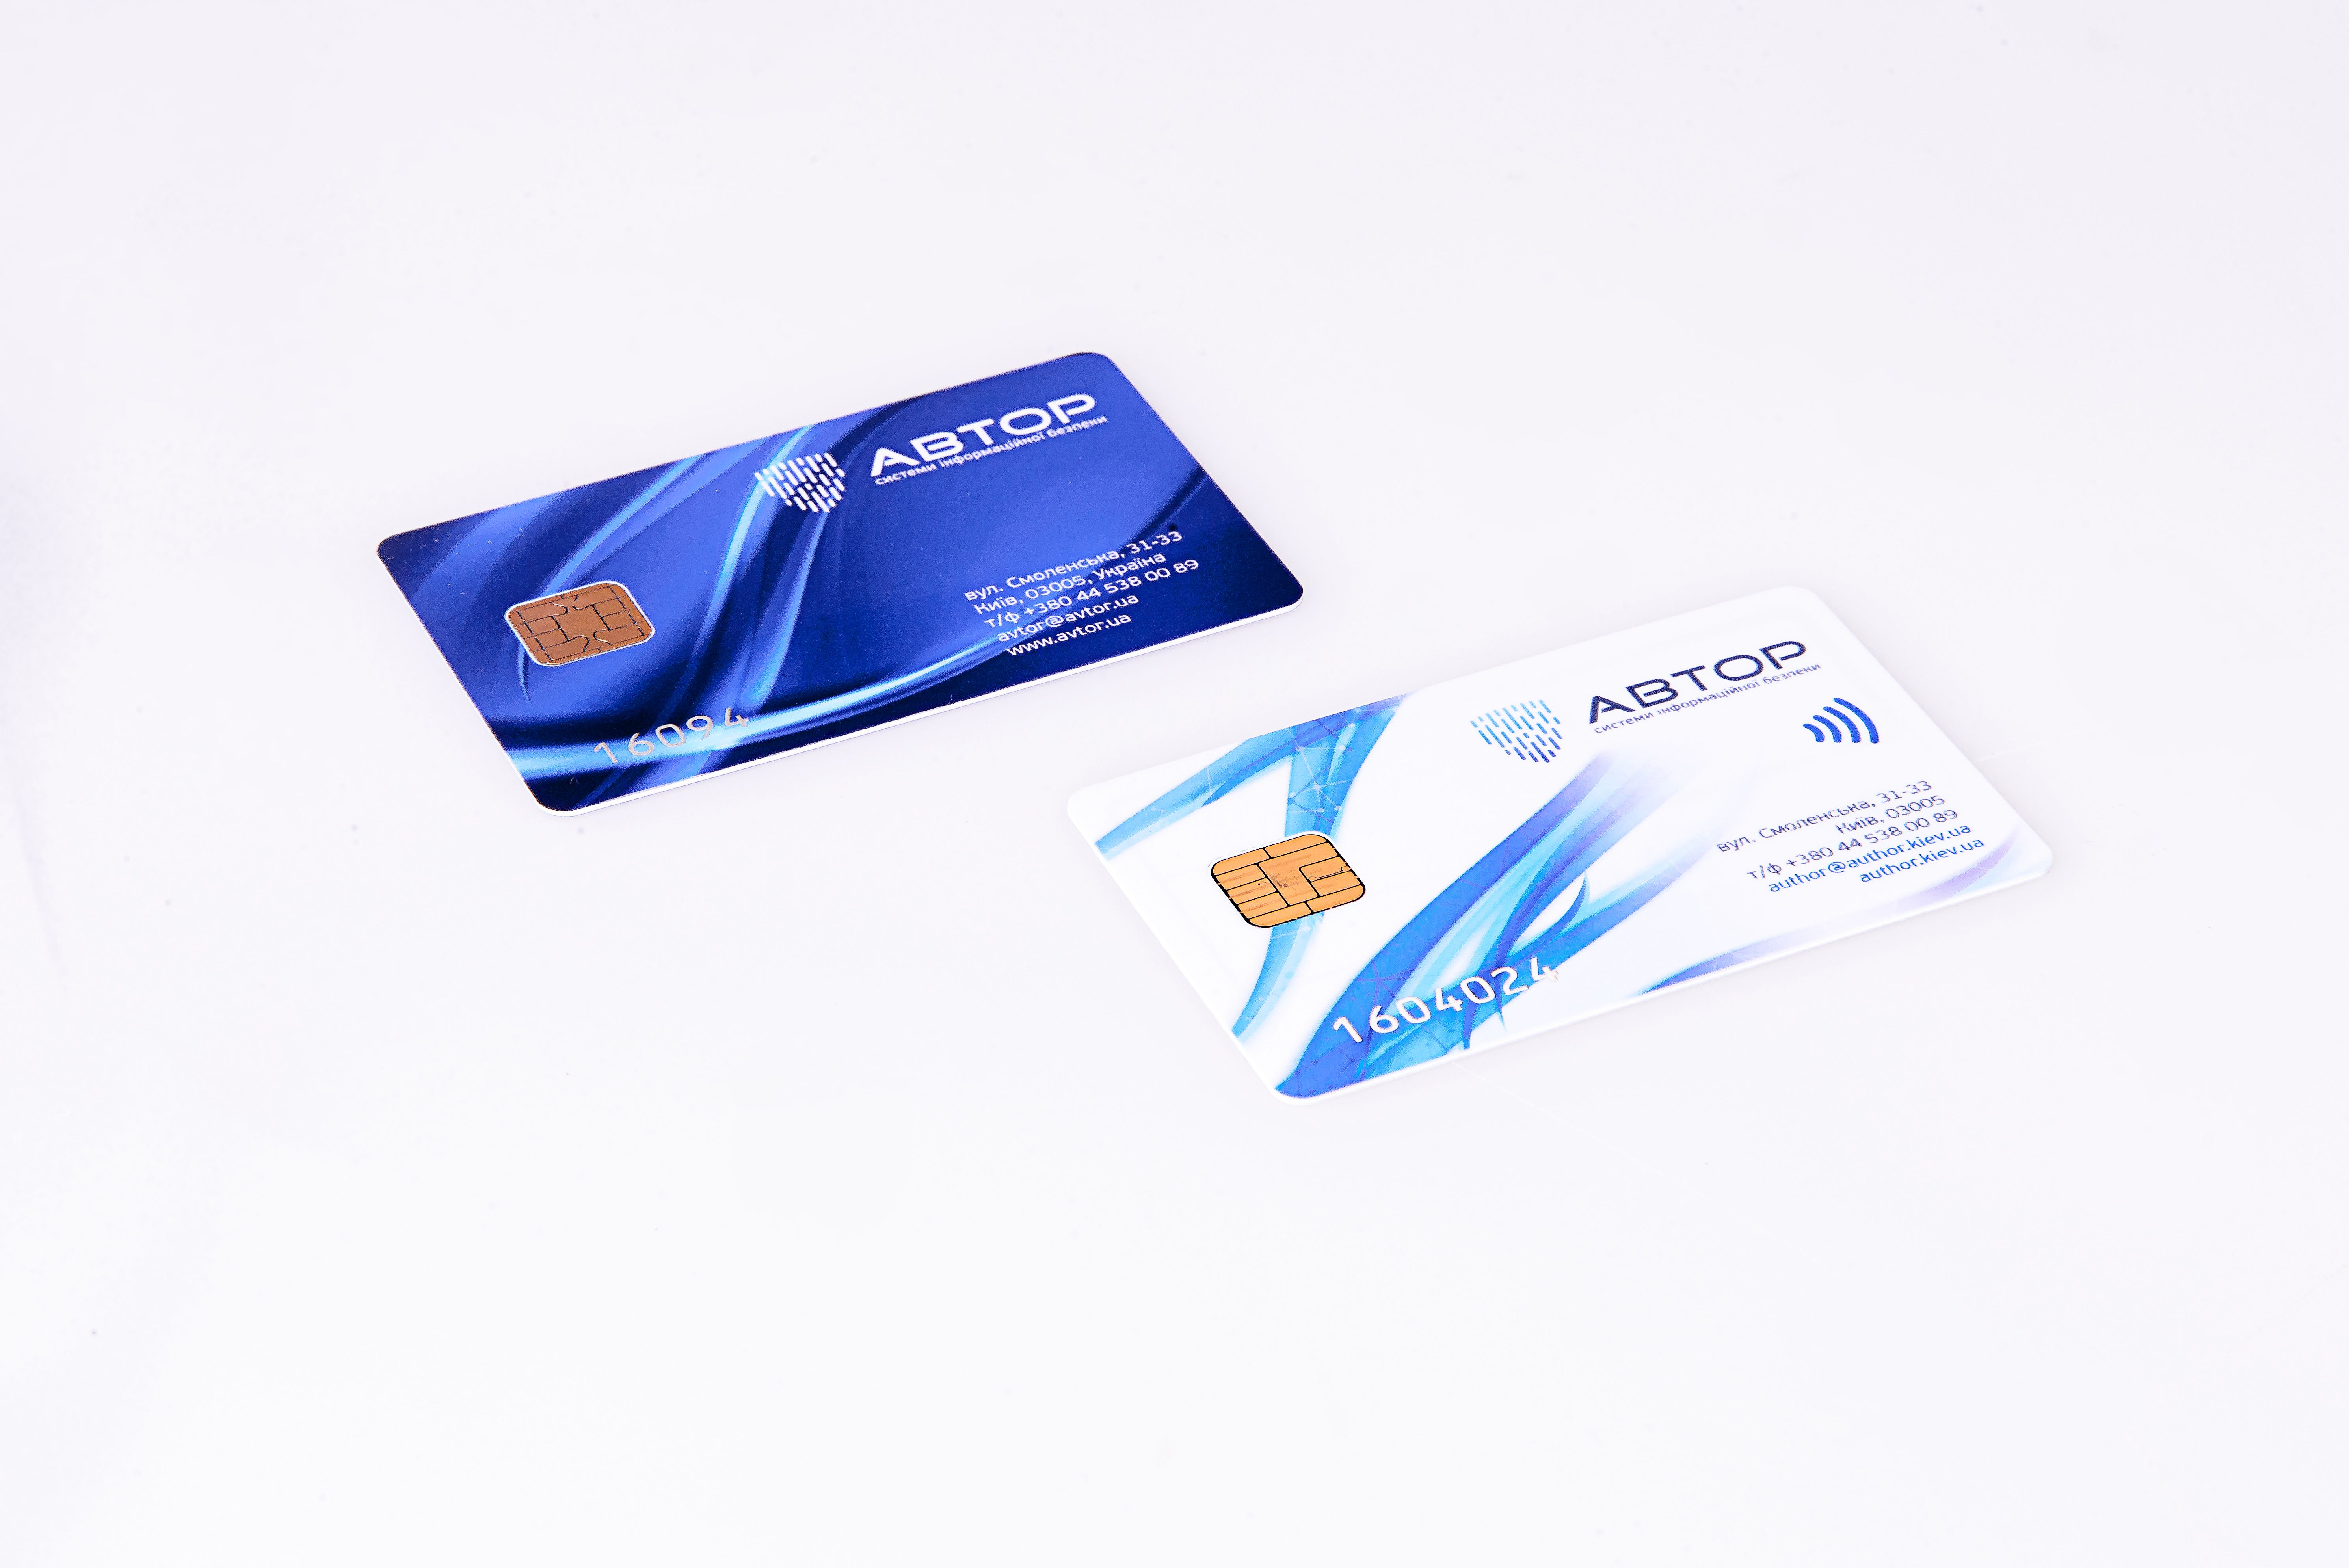
\includegraphics[scale=0.033]{../IMAGES/avtor_smart_cards.jpg}
        \caption{}
        % обратите внимание на знак % после \end{subfigure} и 
        % отсутствие пустых строк и разделителей после \end{subfigure}
        % -- это сливает в одну строку подфигуры
    \end{subfigure}%
    \begin{subfigure}[c]{0.5\textwidth}
        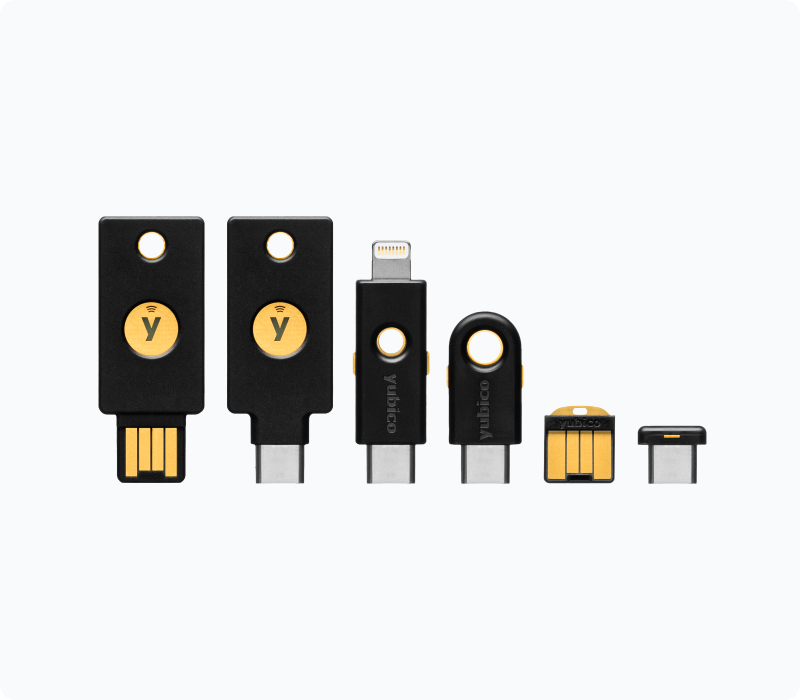
\includegraphics[scale=0.4]{../IMAGES/YubiKey-5.png}
        \caption{}
    \end{subfigure}
 
    \caption{Приклади готових токенів: (a) смарт-картки від Автор, (б) лінійка YubiKey-5 від Yubico.}
    \label{fig_sudak}
\end{figure}


\chapter{Порівняння інтерфейсів Microsoft Crypto API, PKCS11}
\label{chap:theory}

Одразу почнімо із розбору основних інтерфейсів, що використовуються у криптографії. Визначимо спочатку для чого кожен інтерфейс використовується.

\section{PKCS11}

% PKCS11
% https://en.wikipedia.org/wiki/PKCS_11
% https://docs.oasis-open.org/PKCS11/PKCS11-base/v2.40/os/PKCS11-base-v2.40-os.html
% https://thalesdocs.com/gphsm/ptk/5.9/docs/Content/PTK-C_Program/Obj_Classes/data_obj.htm
% https://www.cryptsoft.com/PKCS11doc/STANDARD/pkcs-11.pdf

Стандарт інтерфейсу криптографічного маркера, PKCS11, створений компанією RSA Security і визначає власні інтерфейси програмування для криптографічних маркерів, таких як апаратні криптографічні прискорювачі та смарт-карти.

Почнімо із PKCS11. PKCS11 (або Cryptoki) є одним із стандартів криптографії з відкритим ключем, що відноситься до програмного інтерфейсу для створення та маніпулювання криптографічними токенами, де зберігається сектеринй ключ. Він був створений компанією RSA Security та у 1995 році було опубліковано першу весірю. Сам стандарт є незалежним від платформи API для криптографічних токенів, таких як апаратні модулі безпеки (HSM) і смарт-карти. Цей стандарт використовується у всіх можливих галузях від можливої автентифікації користувача на певній платформі до взаємоції із Центрами Сертифікації.

Основними функціями PKCS11 інтерфейсу моможна назвати:
    \begin{itemize}
        \item шифрування та розшифровування даних;
        \item генерація та перевірка цифрових підписів;
        \item ідентифікація і аутентифікація криптографічного модуля;
        \item управління ключами;
        \item виконання інших криптографічних функцій.
    \end{itemize}

До прикладу використання цього інтерфейсу можна навести приклад роботи із пристроєм від Yubico. Спробуємо вивести та показати сертифікат, що записаний на токен.

\begin{figure}[!h]
    		\centering
    		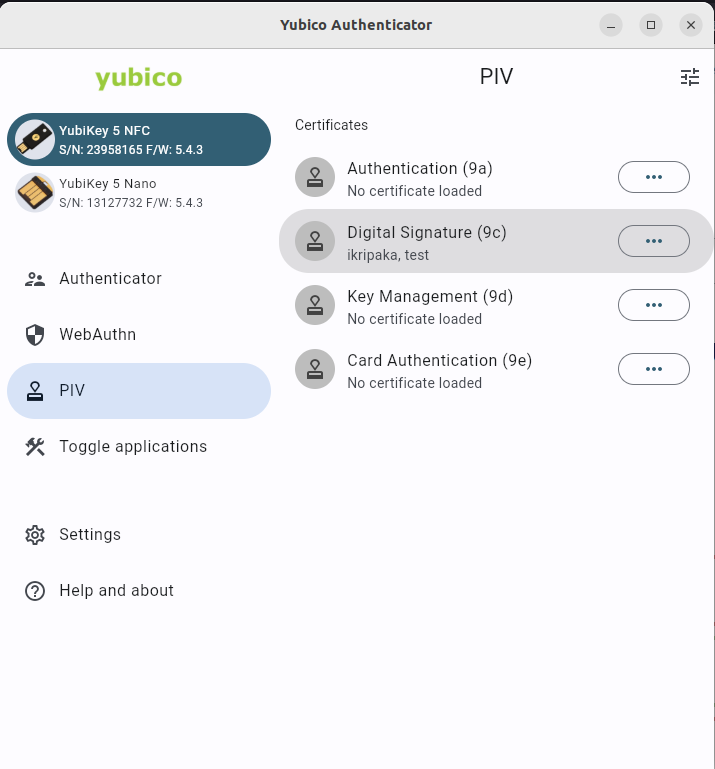
\includegraphics[scale = 0.3]{IMAGES/app_view_main_screen.png}
    		\caption{Головний екран утиліти Yubico authenticator, де видно 2 токени та PIV(Personal Identity Verification).}
    		\label{fig:app_view_main_screen}
	\end{figure}

\begin{figure}[!h]
    		\centering
    		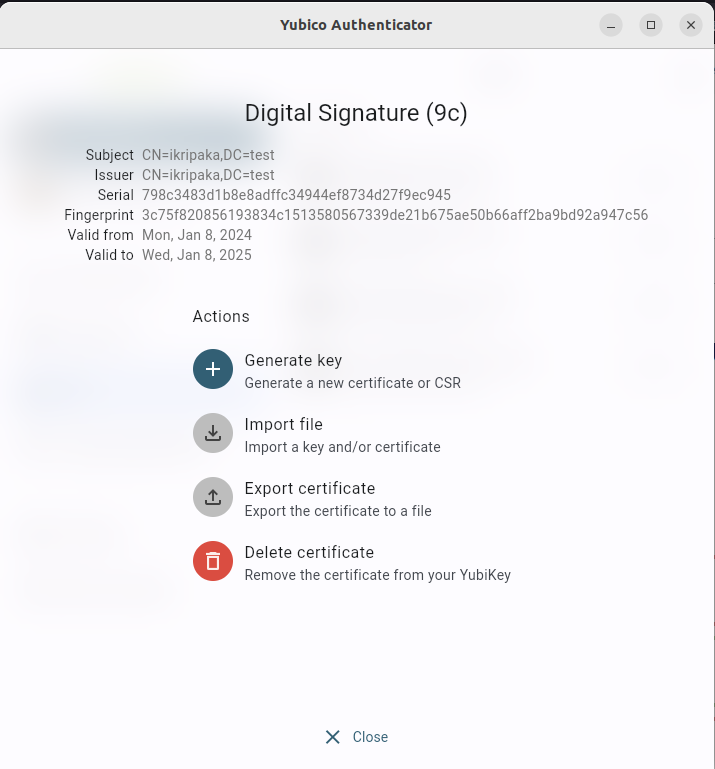
\includegraphics[scale = 0.3]{IMAGES/app_view_token.png}
    		\caption{Переглянемо ідентифікацію юзера за допомогою цифрового підпису.}
    		\label{fig:app_view_token}
	\end{figure}

\begin{figure}[!h]
    		\centering
    		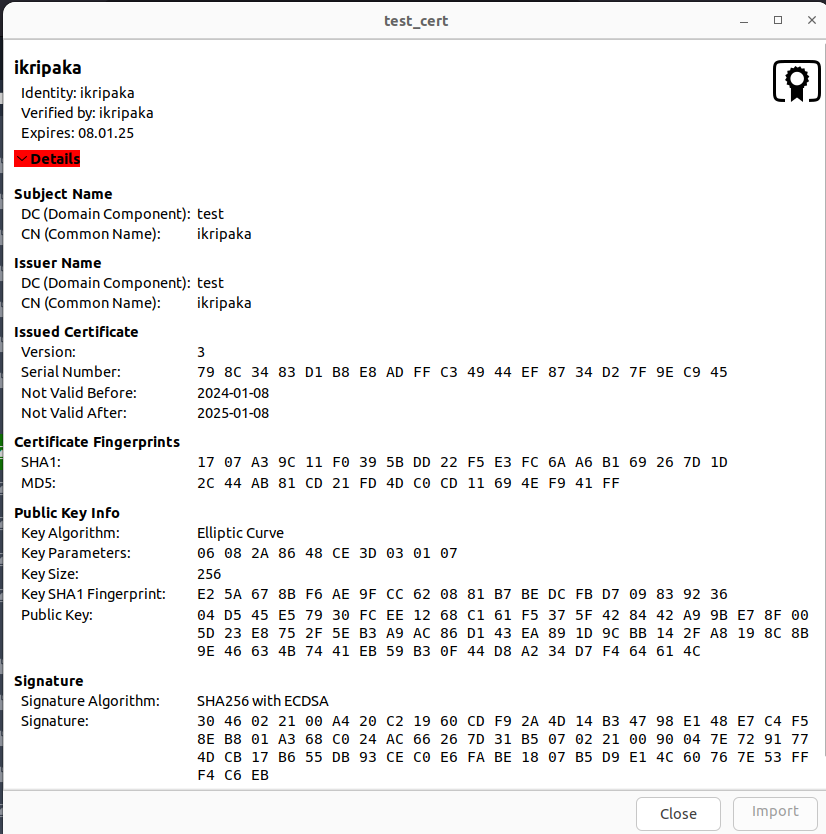
\includegraphics[scale = 0.3]{IMAGES/certicate_view.png}
    		\caption{Вигляд збереженого сертифікату через системний переглядач.}
    		\label{fig:certicate_view}
	\end{figure}

Коментуючи ці картинки можна сказати, що на першій картинці \ref{fig:app_view_main_screen} видно головний екран Yubico Authenticator -- програми, що дозволяє редагувати інформацію токена. Саме у цій версії можна побачити способи ідентифікаціїї. У даному випадку це ті ж WebAuth та PIV.
Щодо другої \ref{fig:app_view_token}, то там видно серійний номер, дату створення/час життя сртифікату. За допомогою можливості зберегти сертитфікат локально його вдалося переглянути і дізнатися як саме було згенеровано його \ref{fig:certicate_view}.

\section{Crypto API}

Взагалі у сфері криптографії існує багато різних криптографічних інтерфейсів, але до заданого API Crypto API можна було знайти два можливих варіанти, один для операційної системи Windows, другий -- для Linux. Розберемо їх та пояснимо різницю між ними. Почнемо із Microsoft CryptoAPI.

\begin{enumerate}       
    \begin{figure}[!h]
    		\centering
    		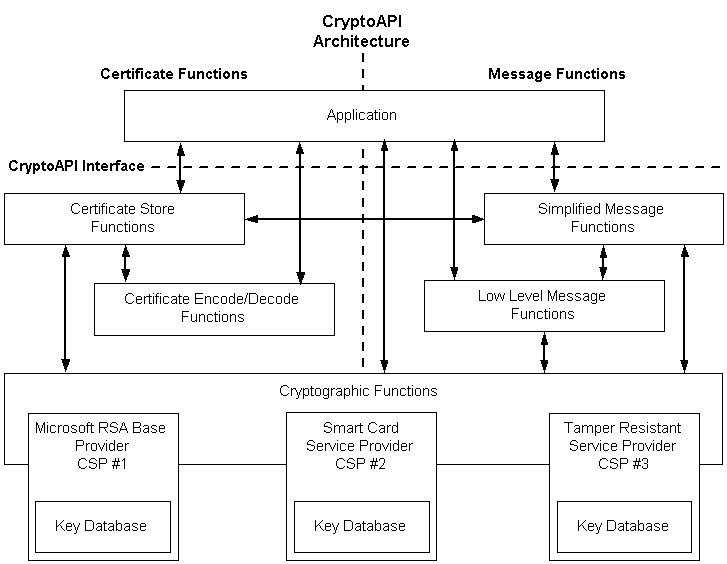
\includegraphics[scale = 0.45]{IMAGES/cryparch.png}
    		\caption{Архітектура побудови CrypytoAPI.}
    		\label{fig:microsoft_crypto_api}
	\end{figure}

    \item Microsoft CryptoAPI
    Microsoft CryptoAPI -- це програмний інтерфейс прикладних програм (API), який надає розробникам Windows-додатків стандартний набір функцій для роботи з криптографією. Він входить до складу операційних систем Microsoft Windows і доступний для використання з простору користувача. Основною фішкою цього API є використання CSP (Cryptographic Service Providers), що є такими собі <<незалежними>> модулями. Тобто архітектура так побудована, що для взаємодії із будь-яким іншим пристроєм або модулем потрібно лише встановити бібліотеку для взаємодії із ним, а CryptoAPI сам зможе звернутися до пристрою і виконати відповідну операцію.
    
    Основними функціями є Microsoft CryptoAPI:
    \begin{itemize}
        \item шифрування та розшифровування даних;
        \item генерація та перевірка цифрових підписів;
        \item алгоритми хеш-функції для перевірки цілісності даних;
        \item захист від сторонніх атак.
    \end{itemize}

    \item Crypto API (Linux)
    Crypto API - це криптографічна структура в ядрі Linux для різних частин ядра, які займаються криптографією, таких як IPsec і dm-crypt. Він був представлений у 2002 році і основною ціллю було забезпечення внутрішніх потреб, однак крім самого ядра користь від нього може отримати і користувач. На даний час він має величезний функціонал із генерування симетричних/асиметричних ключів, взаємодії із різноманітними криптопримітивами. Детальніше можона знайти докумнтацію за \href{https://www.kernel.org/doc/html/latest/crypto/index.html}{покликанням}. 

    \begin{remark}
    
        \begin{itemize}
            \item IPsec --  це набір безпечних мережевих протоколів, який автентифікує та шифрує пакети даних, щоб забезпечити безпечний зашифрований зв’язок між двома комп’ютерами через мережу. Він використовується у віртуальних приватних мережах (VPN).

            \item dm-crypt -- прозора підсистема шифрування блокових пристроїв у ядрі Linux версії 2.6 і пізніших. Воно є частиною інфраструктури пристрою відображення пристроїв і використовує криптографічні процедури з Crypto API ядра.
        \end{itemize}
    \end{remark}
    
\end{enumerate}

\section{Відмінності CryptoAPI від PKCS11 інтерфейсів}

Говорячи про відмінності, то можна їх класифікувати таким чином:

\begin{tabularx}{\textwidth}{X|X|X}
	\textbf{Характеристика} & \textbf{Microsoft CryptoAPI} & \textbf{PKCS11} \\
	      Власність & власність Microsoft & відкритий стандарт \\
        Доступність & простір користувача & простір ядра/простір користувача  \\
        Підтримувані алгоритми & широкий спектр & широкий спектрм \\
        Гнучкість & менш гнучкий & більш гнучкий \\
        Масштабованість & менш масштабований & більш масштабований \\
        Використання &  Windows & Windows, Linux, IOS, Android... \\	
\end{tabularx}

Коментуючи попередню таблицю можна сказати:
\begin{enumerate}

    \item Щодо доступності, то CryptoAPI є історією так само локальною як і в попередньому пункті, але її звичайно можуть використовувати розробники/користувачі для певних потреб. Із іншого боку PKCS11 дає лише інтерфейс, який усі повинні реалізувати, а <<внутрощі>> уже регламентуються виробниками та тим як вони записують дані. 
    \item Не можна не сказати слово про спосіб використання. Ці два порівнювані API можна сказзати взагалі із різних царин. Один використовується на портативних токенах для виконання криптографічниз операцій, а інший є архітектурою побудови/реалізації криптографічних програмних модулів. Такод додам, що сам інтерфейс CryptoAPI доступний лише на пристроях/програмному забезпеченні, що розробляє Microsoft, а, насамперед, PKCS11 стандарт доступний ледь не на кожній ОС. Останній є стандартом індустрії для реалізації HSM, смарт карток, токенів, що повинні використовуватися будь-де на будь-яких пристроях.

\end{enumerate}




% \chapconclude{\ref{chap:review}}

% Наприкінці кожного розділу ви повинні навести коротенькі підсумки по його 
% результатах. Зокрема, для оглядового розділу в якості висновків необхідно 
% зазначити, які задачі у даній тематиці вже були розв'язані, а саме 
% поставлена вами задача розв'язана не була (або розв'язана погано), тому у 
% наступних розділах ви її й розв'язуєте.

% Якщо ваш звіт складається з одного розділу, пропускайте висновок до 
% нього~-- він повністю включається в загальні висновки до роботи